\documentclass[12pt,a4paper,oneside]{article}
\usepackage{fullpage}
\usepackage[none]{hyphenat} 
\usepackage{natbib}
\usepackage{algorithm}
\usepackage{algorithmic}
\usepackage{graphicx}

\newcommand{\HRule}{\rule{\linewidth}{0.5mm}}


\begin{document}

\begin{titlepage}
    \begin{center}
        \textsc{\large Eastern Michigan University}\\[1.5cm]
        \textsc{\large Computer Science Department}\\
        \textsc{\large Masters Thesis Proposal}\\[0.5cm]
        \HRule\\[0.4cm]
        { \huge \bfseries  Realtime Raytracing }\\[0.4cm]
        \HRule\\[1.5cm]

        % Author and supervisor
        \begin{minipage}{0.45\textwidth}
            \begin{flushleft} \large
                \emph{Author:}\\
                Byron \textsc{Heads} \\
                \small Eastern Michigan University\\
                \small Computer Science Department \\
            \end{flushleft}
        \end{minipage}
        \begin{minipage}{0.45\textwidth}
            \begin{flushright} \large
                \emph{Thesis Advisor:} \\
                Dr.~William \textsc{Sverdlik}\\
                \small Eastern Michigan University\\
                \small Computer Science Department
            \end{flushright}
        \end{minipage}

        \vfill
        %{ \large \textbf{Abstract Summary}}\\
    
        \HRule\\[0.5cm]
        { \large \today }
    \end{center}
\end{titlepage}

\begin{abstract}



\end{abstract}
\newpage 
\tableofcontents
\newpage 

\section{ Introduction }

Computer graphics used in modern games and simulation environments are based around the \textbf{z-buffering} algorithm.  Z-buffering builds a scene by computing the depth of triangles in a scene from the from a view-point,  to as the \textbf{eye}.  The algorithm is simple and each pixel can be computed with stream processors that are commonly  used on modern GPUs.  Hardware implementations of z-buffers commonly have two frame buffers for a color and a depth buffer.    The color buffer is split into the front buffer and the back buffer.  The back buffer is where the algorithm is rendering to, and the front buffer is drawn to the screen.  Once the back buffer it filled it is swapped with the front buffer, this is normally done with a simple pointer swap.  The algorithm for z-buffer is as follows \cite{fast:2008}:

\begin{algorithm}
\begin{algorithmic}[1]
\STATE $C[ ] \gets \textit{background color}$ 
\STATE $Z[ ] \gets \infty$
\FOR{ all \textit{N} triangles }
	\FOR{ each pixel p in triangle }
		\STATE $c \gets \textit{new color}$
		\STATE $z \gets \textit{new depth}$
		\IF{ $z < Z_{p} $ }
			\STATE $Z_{p} \gets z$
			\STATE $C_{p} \gets c$
		\ENDIF
	\ENDFOR
\ENDFOR
\end{algorithmic}
\caption{Example of the z-buffer algorithm}
\label{z-buffer}
\end{algorithm}

This algorithm works by tracking the depth of the color for each given pixel that is rendered in the back buffer.  This algorithm is fast and easy to implement but nowhere in the algorithm is light, shadow, reflection, or refraction calculated.  To produce these effects simple ray casting needs to be added to the z-buffer algorithm, but a z-buffer only accounts for testing distance from a single point, the eye, but to test for objects in shadow or to calculate reflection the algorithm needs to be able to work from any point in space.  The solution relies in building a better physics model for light.

To make a better model we first need to understand how light works.  In the real world light source emit photons that collide with an object which changes the energy state of the photon.  This photon is then reflected off of the object and then enters into the lens of our eye.  From there our brain interpreters this as color.  One problem with this model is that only a very small percent of the emitted light is actually seen, most of the computations are wasted and never used.  A better solution exists in ray tracing.  

A more efficient way to model realistic light is to trace photons that enter the eye back to sources of light.  Furthermore each photon can be computed independently of each other making ray tracing inherently parallel in nature.  An initial point is used as the light focal point, this is known as the \textit{eye}.  A photon is traced backwards from the eye through an image plane that is in front of the eye.  This image plane acts like film in a pinhole camera.  

\begin{figure}[H]
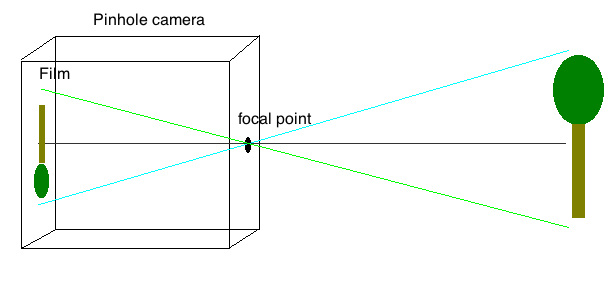
\includegraphics[scale=0.6]{pineholecamera.png} 
\caption{Pinhole camera}
\label{pinhole-camera}
\end{figure}

In a pinhole camera the image is upside down on the film because the photons pass through the focal point and cross the center plain.  The camera can be simplified by moving the film in front of the focal point.

 \begin{figure}[H]
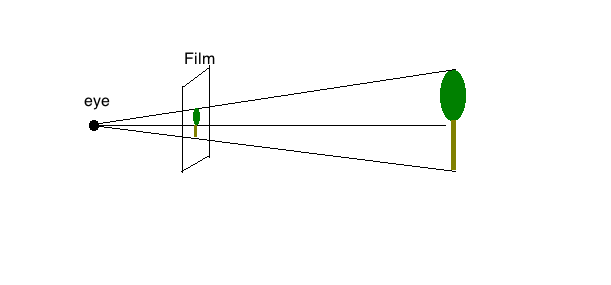
\includegraphics[scale=0.6]{raycamera.png} 
\caption{Ray tracer camera}
\label{ray-camera}
\end{figure}

Algorithm \ref{ray-trace} is a simple implementation that works fairly similar to the z-buffering algorithm.  The scene consists on a list of geometric  objects.  Any shape that ray-object collision can be detected can be used.  The image buffer is an array that holds the resulting output from the algorithm.  A ray consists of a starting point and a normalized direction.  A ray is created at the eye, in the direction of each pixel in the image plane.  The color of the pixel is set to the color of the closest object that the ray collides with.  A simple ray tracer can be made with the following algorithm:

\begin{algorithm}[H]
\begin{algorithmic}[1]
\STATE $O[ ] \gets \textit{All objects in scene}$ 
\STATE $I[] \gets 0$ \COMMENT{Clear image buffer}
\STATE
\FOR{ each pixel p in I }
	\STATE $I_{p} \gets raytrace( castray( eye, p ))$
\ENDFOR
\STATE 
\STATE \textit{color} \textbf{function} raytrace(  R )
	\STATE $c  \gets \textit{ambient color } $
	\STATE $d \gets \infty $
	\FOR{ each object o in O[] }
		\IF{ collision( R, o )  }
			\IF{ $distance( \textit{eye}, o ) < d$ }
				\STATE $d \gets distance( \textit{eye}, o )$
				\STATE $c \gets color( o )$
			\ENDIF
		\ENDIF
	\ENDFOR
	\STATE \textbf{return} c

\end{algorithmic}
\caption{Simple ray tracing algorithm}
\label{ray-trace}
\end{algorithm}

Adding light and shadow to this algorithm is done by computing the light at each collision point.  At each point of collision a ray is casted from that point to each light in the scene.  If their is not an object between the collision point and the light then the point is considered in light, else it is in shadow.  The color of a point is computed from three components: \textit{ambient}, \textit{diffuse}, and \textit{specular} \cite{kalinini:2008}.

Surfaces can be made reflective or refractive by using the recursive nature of ray tracing.  If a surface is reflective, a new ray is computed at the ray collision point using the surface normal at that point as the reflection plane.  The tracing algorithm can be called with the ray.  Refraction is handled in the same way with the exception of the way the refracted ray is computed.  Algorithm \ref{ray-trace-full} shows an example of lighting, reflections, and refractions.  
  

\begin{algorithm}[H]
\begin{algorithmic}[1]
\STATE $O[\ ] \gets \textit{All objects in scene}$ 
\STATE $L[\ ] \gets \textit{All lights in scene}$
\STATE $I[\ ] \gets 0$ \COMMENT{Clear image buffer}
\STATE
\FOR{ each pixel p in I }
	\STATE $I_{p} \gets raytrace( castray( eye, p ))$
\ENDFOR
\STATE 
\STATE \textit{color} \textbf{function} raytrace(  R, depth )
	\STATE $c  \gets \textit{ambient color } $
	\STATE $d \gets \infty $
	\STATE $s \gets \textit{NULL}$
	\FOR{ each object o in O[] }
		\IF{ collision( R, o )  }
			\IF{ $distance( \textit{eye}, o ) < d$ }
				\STATE $d \gets distance( \textit{eye}, o )$
				\STATE $s \gets o$
			\ENDIF
		\ENDIF
	\ENDFOR
	\IF{ $s\ \textbf{NOT}\ \textit{NULL}$ }
		\STATE \COMMENT{Find direct light on object s}
		\STATE $pi \gets pointOfCollision( R, s )$
		\FOR{ each light l in L }
			\STATE $lr \gets castRay( pi, l )$
			\STATE $ld \gets distance( pi, l )$
			\STATE $shade \gets 1$
			\FOR{ each object o in O }
				\IF{ collision( lr, o ) \textbf{AND} distance( lr, o ) < ld }
					\STATE $shade \gets 0$				
				\ENDIF
				\STATE $c \gets c +( diffuse( s, l ) + specular( s, l )) * shade$ 
			\ENDFOR
		\ENDFOR
		\STATE \COMMENT{Recursively compute reflections}
		\IF{ $reflectivity( s ) > 0\ \textbf{AND}\ depth < depthMax$ }
			\STATE $rr \gets reflection( pi, normal( s, pi ))$
			\STATE $c \gets c + raytrace( rr ) * reflectivity( s )$
		\ENDIF
		\STATE \COMMENT{Recursively compute refraction}
		\IF{ $transparency( s ) > 0\ \textbf{AND}\ depth < depthMax$ }
			\STATE $rr \gets refraction( pi, normal( s, pi ), s )$
			\STATE $c \gets c + raytrace( rr ) * transparency( s )$
		\ENDIF
	\ENDIF
	\STATE \textbf{return} c

\end{algorithmic}
\caption{ Ray tracing algorithm with lighting }
\label{ray-trace-full}
\end{algorithm}

The images produced with this algorithm produces sharp edges around objects and shadows.  The image is to sharp to be natural, to clean up the image anti aliasing and soft shadows need to be added.  Adding anti aliasing is done by casting more rays through a pixel and averaging the resulting colors together.  To do this the area in space that the pixel covers needs to be subdivided into smaller regions.  A ray is cast from the eye through these regions.  The ray can be cast through the center for a shaper image, or randomly for softer edges.  Anti aliasing can increase the computation cost dramatically.  Splitting a pixel into quarters increases the computation cost by four times.

\begin{figure}[H]
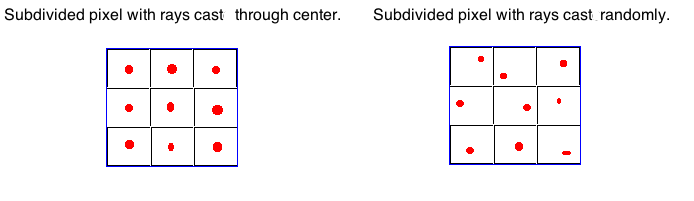
\includegraphics[scale=0.6]{aa.png} 
\caption{Anti aliasing for a single pixel.}
\label{aa}
\end{figure}

Soft shadows are used to make a softer transition from light to shadow.     The simple lighting model cast a ray from the collision point to the center of a light, but for points that are on the edge of a shadow may get partial light.  In the real world a light bulb has volume.  A soft shadow is computed by casting several rays from the collision point to a point in the lights volume, the results are averaged together to computer the finial color.


\begin{figure}[H]
\begin{center}
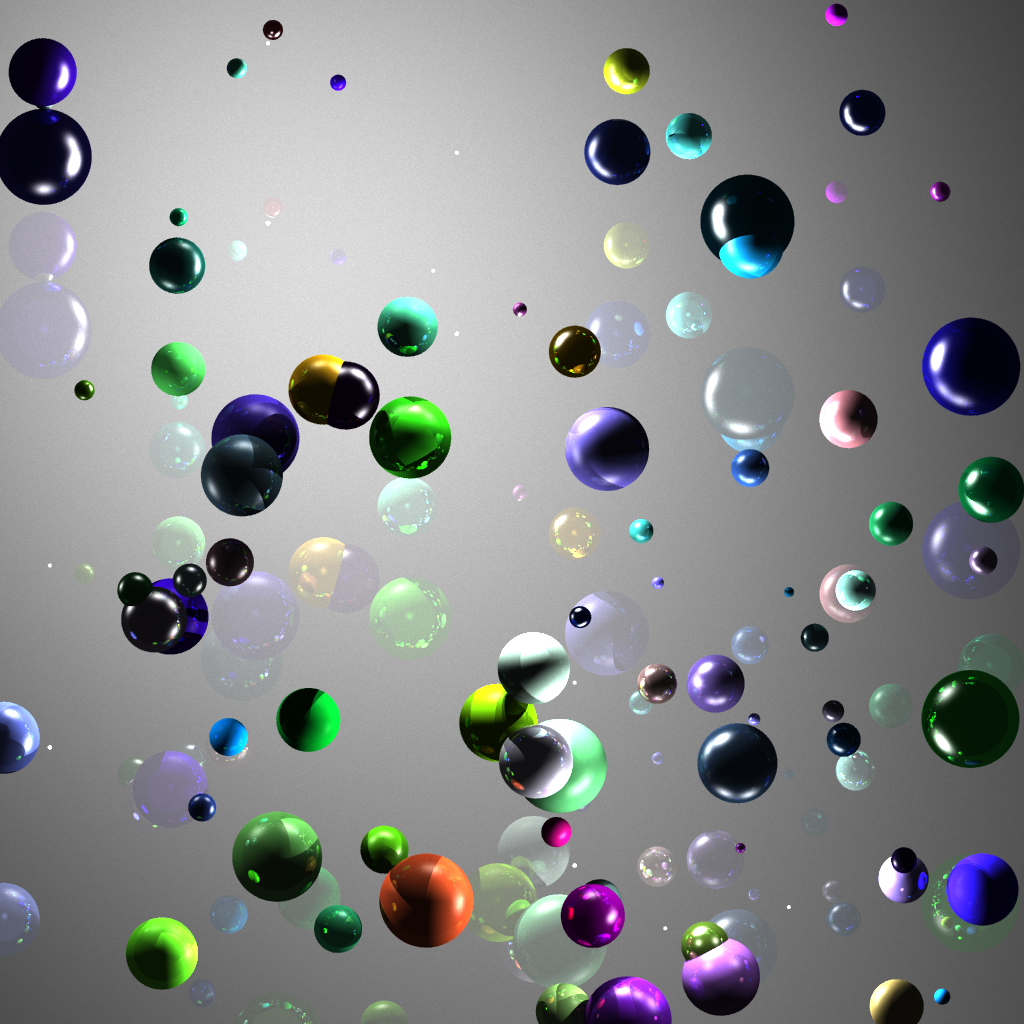
\includegraphics[scale=0.35]{result1.png} 
\caption{Non-optimized ray traced image with 8 light, and 80 spheres.  34 minuet render time.}
\label{result1}
\end{center}
\end{figure}


\newpage
\listofalgorithms
\listoffigures
\listoftables
\bibliographystyle{plain}
\bibliography{proposal}

\end{document}

